\chapter{Objetivos} \label{cap:Objetivos}
%\section{Objetivos} \label{s:objeticos}
%\pagenumbering{arabic}
%\setcounter{page}{1}

%\setcounter{section}{2}

En el siguiente capítulo se detallarán las metas concretas que se pretenden alcanzar en este Trabajo Fin de Máster.

\section{Objetivos}
Desde el nacimiento de Visual SLAM, se están desarrollando algoritmos que permitan a los robots estimar su posición, o con una cámara localizar una imagen en tiempo real en 3D para aplicaciones de realidad aumentada. Estos algoritmos son complejos y están compuestos de múltiples etapas, a menudo un ligero cambio en alguna de estas etapas puede hacer que los resultados del algoritmo mejoren significativamente o por el contrario empeoren. Sería muy útil y conveniente contar con una herramienta que permitiese analizar o estimar la bondad de los nuevos algoritmos Visual SLAM.

\textbf{El objetivo principal de este proyecto es presentar una herramienta que permita comparar cuantitativamente el rendimiento de los algoritmos Visual SLAM y la calidad de sus estimaciones}.

Esta herramienta permitirá comparar el rendimiento de los diferentes algoritmos de Visual SLAM así como estudiar más fácilmente que modificaciones o mejoras se podrían aplicar en los algoritmos ya existentes.

En  este TFM nos hemos centrado en medir la exactitud de las estimaciones de posición sin tener en cuenta la generación de mapas, es decir se ha puesto toda la atención en comparar las mediciones de \textit{tracking} dejando el \textit{mapping} para futuros proyectos. 

Entenderemos que un algoritmo A es mejor que otro B cuando el algoritmo A sea capaz de estimar la posición con mayor exactitud que otro algoritmo B en el menor tiempo posible y de manera robusta. La herramienta a desarrollar medirá la precisión de las estimaciones de posición y la agilidad entendiéndose esta como el tiempo de proceso dedicado a realizar dichas estimaciones de posición. 

Típicamente esta herramienta permitirá comparar dos secuencias de posiciones 3D, la estimada por un algoritmo de Visual SLAM y la secuencia de posiciones verdaderas. La diferencia entre ambas mide el error del algoritmo SLAM a la hora de estimar correctamente las posiciones de la cámara.
Este objetivo principal lo hemos articulado en los siguientes subobjetivos:

\begin {enumerate}
\item \textbf{Conseguir un Registrador Espacial:} Este registrador espacial debe permitir registrar 2 secuencias de puntos 3D en el espacio, estimando rotación, traslación y escala para poder realizar el registro espacial entre las 2 nubes de puntos.


\item \textbf{Registrador Temporal:} Que permita sincronizar las 2 secuencias de puntos 3D. Para ello deberemos ajustar los 2 secuencias a la misma frecuencia de muestreo, (utilizaremos interpolación) y también calcular el offset temporal entre ambas. El offset temporal sería la diferencia de tiempo entre 2 secuencias. 

\item \textbf{La herramienta de medición se validará experimentalmente:} Para comprobar que funciona correctamente realizaremos experimentos donde comprobaremos el error estimado entre la verdad absoluta (groundtrouth) y una secuencia transformada de la que se conoce exactamente el registro temporal y espacial. Se creará un Módulo de Transformación que permitirá realizar tanto alteraciones temporales como espaciales a una secuencia dada generando como resultado una nueva secuencia transformada.

\end {enumerate}

\section {Requisitos}

La solución que se desarrolle para alcanzar los objetivos deberá satisfacer además estos requisitos:


	\textbf{R1}. La herramienta debe restringirse a la comparación de algoritmos Visual SLAM que utilizan como sensor de visión una cámara RGB. Así quedan descartados los algoritmos que emplean cámaras RGBD.

	\textbf{R2}. Se restringirá solo a los algoritmos Visual SLAM que empleen \textit{una sola} cámara.

	\textbf{R3}. La herramienta debe ser aplicable a nuevos algoritmos de Visual SLAM.

	\textbf{R4}. Facilidad de uso.

	\textbf{R5}. Debe ofrecer una única métrica cuantitativa para la comparación entre varios algoritmos de Visual SLAM.

	\textbf{R6}. Debe ofrecer resultados fácilmente legibles y reconocibles para el usuario.

	\textbf{R7}. El software generado debe ser abierto y estar públicamente disponible.

\section{Metodología y plan de trabajo}

En cuanto a la metodología utilizada para desarrollar este TFM, se ha seguido el modelo de ciclo de vida en espiral. Una de las primeras lecciones que se aprenden de las metodologías ágiles es que la metodología debe adaptarse al proyecto y no al revés. Dicha premisa cobra más importancia en un proyecto realizado por una sola persona.

\begin{figure}[H]
\begin{center}
\label{fig:espiral}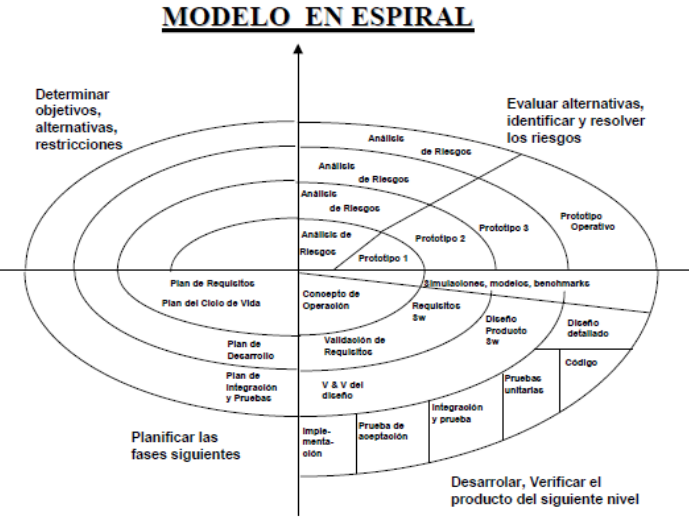
\includegraphics[height=6.0cm]{img/cap2/modeloEspiral.png}
\end{center}
\caption{Inicialización de Mono SLAM con 4 puntos conocidos.}
\end{figure}


El modelo en espiral es un modelo iterativo, donde cada ciclo viene a representar una fase del proyecto software. Podemos diferenciar 4 fases dentro de cada ciclo del modelo en espiral

\textbf{-Determinar los Objetivos:} Determinaremos que metas se deben conseguir en cada iteración, teniendo en cuenta los objetivos del proyecto.

\textbf{-Evaluación de alternativas:} Evaluar las distintas alternativas para alcanzar las metas que se han establecido en la fase anterior, utilizando distintos puntos de vista.

\textbf{-Desarrollo y Evaluación:} Una vez seleccionada la mejor alternativa, se diseña y desarrolla el producto y por último se realizarán pruebas para testear su funcionamiento.

\textbf{-Planificación:} Teniendo en cuenta los resultados de las pruebas realizadas, se planificará la siguiente iteración revisando posibles errores cometidos en iteraciones anteriores y se comienza con una nuevo ciclo en espiral.

Por consiguiente, y enmarcándolo dentro de la metodología en espiral, primero se ha realizado un estudio previo muy amplio que sirve para obtener una visión completa del problema de Visual SLAM y detectar puntos críticos. Segundo se ha ido acotando hasta el primer prototipo del desarrollo principal, el cual ha sido revisado y validado en varias iteraciones. Este prototipo inicial es importante ya que no sólo nos permite avanzar en todas las vías en paralelo, sino porque ofrece una prueba de concepto para las ramificaciones que se han paralizado en favor del desarrollo troncal.

El proceso de desarrollo ha sido supervisado por los tutores mediante tres herramientas: reuniones semanales, definición de hitos y diario de trabajo.
Durante las reuniones se debían definir varios hitos de corto o medio plazo en los que se trabajaría esa semana. Este progreso se puede ver en la página web habilitada para tal uso:
\footnote{https://jderobot.org/Elias-tfm}

Así mismo, el código fuente desarrollado puede encontrarse en \footnote{https://github.com/JdeRobot/slam-Testbed} y la memoria en \footnote{https://github.com/RoboticsURJC-students/2017-tfm-elias-barcia}

\clearpage
\newpage
\pagebreak


